\documentclass[conference]{IEEEtran}
\IEEEoverridecommandlockouts

\usepackage{amsmath,amssymb,amsfonts}
\usepackage{algorithmic}
\usepackage{graphicx}
\usepackage{textcomp}
\usepackage{xcolor}
\usepackage{booktabs}
\usepackage{url}
\usepackage{cite}
\usepackage{tikz}
\usetikzlibrary{arrows.meta, positioning, calc, shapes.geometric, fit, backgrounds, decorations.pathreplacing}

% Shared notation macros
% IntelliTwin Shared Universal Mathematical Notation Macros
% Source of Truth: research/research_design/statistical_inference_protocol.md
% Pinned Repository Commit: bb9e34579343881a831e3f052608ee15e183df76

\usepackage{amsmath,amssymb}

% Primary maintenance cost metrics (Simulated Cost Units - SCU)
\newcommand{\SCU}{\text{SCU}}
\newcommand{\Cost}{\text{Cost}}
\newcommand{\CPM}{C_{\text{PM}}}
\newcommand{\CFAIL}{C_{\text{FAIL}}}
\newcommand{\CWASTE}{C_{\text{WASTE}}}
\newcommand{\MPIW}{\text{MPIW}}
\newcommand{\RUL}{\text{RUL}}

% Decision and effect size contrasts
\newcommand{\Deltacost}{\Delta_{\text{cost}}}
\newcommand{\Deltaerror}{\Delta_{\text{error}}}
\newcommand{\Deltafail}{\Delta_{\text{fail}}}
\newcommand{\Dwidth}{D_{\text{width}}}
\newcommand{\Dscore}{D_{\text{score}}}

% Subgroup and worst-group indicators
\newcommand{\WorstErr}{\text{WorstErr}}
\newcommand{\WorstRegime}{\text{WorstRegime}}
\newcommand{\WorstStage}{\text{WorstStage}}

% Interval bounds and predictions
\newcommand{\RULtrue}{y}
\newcommand{\trueRUL}{y}
\newcommand{\cappedRUL}{y_{\text{cap}}}
\newcommand{\RULpred}{p}
\newcommand{\LowerBound}{L}
\newcommand{\UpperBound}{U}

% Quantile thresholds
\newcommand{\qglobal}{q_{\text{global}}}
\newcommand{\qregime}{q_k}
\newcommand{\qfinal}{q^*}

% Asymmetric shape and scaling functions
\newcommand{\sigmap}{\sigma(p)}
\newcommand{\zp}{z(p)}
\newcommand{\ap}{a(p)}
\newcommand{\bp}{b(p)}


\begin{document}

\title{IntelliTwin: Asymmetric, Condition-Adaptive Conformal Prediction for Industrial Turbofan Predictive Maintenance\\
\thanks{This research draft reflects prespecified methodology and protocol specifications frozen under commit \texttt{c163bb279e7427b8f1b6e75955af4969ff9370fd} (Audit Execution: \texttt{550a7994d5746d3bcbfa28c26e7ed4f1a26a6153}). Author ordering, formal affiliations, and individual contributions remain pending team agreement. Held-out experimental results are blinded and pending completion of experimental verification gates (UPD-02, UPD-03, UPD-04).}
}

\author{
\IEEEauthorblockN{Mayank Singh}
\IEEEauthorblockA{IntelliTwin Research Initiative \\
Email: \textit{pending-institutional-records}}
\and
\IEEEauthorblockN{Shiksha Pandey}
\IEEEauthorblockA{IntelliTwin Research Initiative \\
Email: \textit{pending-institutional-records}}
\and
\IEEEauthorblockN{Ruchi Gupta}
\IEEEauthorblockA{IntelliTwin Research Initiative \\
Email: \textit{pending-institutional-records}}
}

\maketitle

\begin{abstract}
Predictive maintenance for industrial gas turbine engines requires timely, risk-calibrated replacement decisions to prevent catastrophic in-flight failures while minimizing premature overhaul costs. Conventional Remaining Useful Life (RUL) prognostic systems rely on point regression models that optimize cycle-level accuracy metrics without quantifying predictive uncertainty or aligning with asymmetric maintenance cost structures. 

In this work, we present \textbf{IntelliTwin}, a framework integrating data-driven base predictors (Gradient Boosted Regressors and Long Short-Term Memory networks) with hierarchical, decision-aware conformal prediction. IntelliTwin enforces strict engine-level disjoint data partitioning, causal temporal windowing ($w=30$, stride 1), equal engine weighting across all evaluations, and condition-stratified conformal calibration. By incorporating an asymmetric loss parameter ($\beta = -\ln 2$), the framework modulates nonconformity scores to reflect the severe cost penalties of component failure relative to preventive replacement. 

We formalize an experimental evaluation protocol across NASA C-MAPSS sub-datasets FD001, FD002, and FD004, comparing calibrated lower bounds against four distinct matched-conservatism baselines across three families. Statistical significance is evaluated via paired engine-cluster bootstrap inference ($B=10{,}000$) with prespecified practical-effect margins and Bonferroni family-wise error rate control ($98.75\%$ confirmatory confidence intervals). 

\textit{Provisional Status Statement:} Base predictors and conformal calibrators are implemented and frozen. The committed v4 pre-test audit reports PASS and PRETEST\_READY. Held-out execution has not started, and RQ1--RQ4 outcomes remain pending. Development validation and audit results do not establish confirmatory maintenance benefit, subgroup reliability, or robustness. Empirical evaluation on the held-out test splits remains pending experimental execution under stable update gates UPD-02, UPD-03, and UPD-04.
\end{abstract}

\begin{IEEEkeywords}
Predictive Maintenance, Conformal Prediction, Remaining Useful Life, Turbofan Engines, Digital Twin, Asymmetric Loss, C-MAPSS.
\end{IEEEkeywords}

\section{Introduction}
\label{sec:introduction}

In safety-critical cyber-physical systems, such as commercial aviation turbofan engines, unexpected component failure incurs catastrophic operational, financial, and life-safety hazards. Consequently, industrial fleet operators have historically adhered to rigid preventive maintenance schedules, overhauling major subsystems at fixed operational intervals (flight hours or cycles). While preventive scheduling mitigates catastrophic in-flight failure, it imposes severe economic costs by routinely discarding components with substantial remaining physical life~\cite{saxena2008damage,shehadeh2024evaluating}.

Predictive Maintenance (PdM) leverages onboard multi-sensor telemetry to transition from time-based maintenance to condition-based, opportunistic intervention. Machine learning prognostics aims to estimate the Remaining Useful Life (RUL) of degrading machinery, enabling timely maintenance before failure occurs. In recent years, deep neural architectures—including Convolutional Neural Networks (CNNs), Long Short-Term Memory (LSTM) recurrent networks, and gradient-boosted decision trees—have achieved remarkable point-prediction accuracy on standardized benchmarks such as NASA C-MAPSS.

However, deterministic point predictors $\hat{y}$ provide no quantification of predictive uncertainty. In sequential decision environments, a deterministic forecast is fundamentally incomplete: an operator cannot determine whether a predicted life of $\hat{y} = 15$ cycles carries high confidence or a substantial probability of immediate breakdown at cycle 2. Furthermore, standard models are trained under symmetric loss functions (such as Mean Squared Error), which penalize early and late errors equally. In physical operations, this symmetry is catastrophic: predicting that an engine will survive longer than it actually does ($d > 0$) risks uncontained in-service failure, whereas predicting failure prematurely ($d < 0$) merely incurs early maintenance cost~\cite{chen2022data,diao2026turbofan}.

To provide principled uncertainty bounds, prognostic models must emit calibrated prediction intervals $[L(x), U(x)]$ targeting nominal coverage $1 - \alpha$. Predictive uncertainty methods differ in their assumptions and calibration behavior. Their maintenance value must be evaluated through interval reliability and downstream decision outcomes under a common protocol. Conformal prediction~\cite{javanmardi2023conformal} provides a distribution-free uncertainty framework.

IntelliTwin uses an engine-weighted conformal construction motivated by hierarchical conformal prediction. Formal coverage results require the hierarchical sampling and exchangeability assumptions stated in the underlying theory. Equal engine weighting does not establish these assumptions for ordered, lifetime-stratified degradation trajectories. This study therefore evaluates marginal and subgroup coverage empirically. It does not claim guaranteed coverage for each engine, lifecycle stage, operating regime, complete trajectory, or adaptively selected maintenance time. Nominal 90% coverage is a target, not a guaranteed realized coverage proportion. Maintenance outcomes are evaluated separately under the frozen simulator.

Despite this theoretical appeal, applying conformal prediction to industrial asset prognostics reveals critical research challenges:
\begin{enumerate}
  \item \textbf{Autocorrelated Degradation Trajectories}: Telemetry cycles within an engine violate observation-level exchangeability. Standard pooled conformal prediction over-weights long-lived engines, introducing survivor bias. Hierarchical, engine-weighted quantile computation~\cite{lee2023hierarchical} balances weight across engine clusters, but finite-sample reliability under trajectory autocorrelation requires empirical validation.
  \item \textbf{Subgroup Reliability Breakdown}: Global conformal calibrators target marginal coverage averaged across all operating cycles, but frequently exhibit acute localized undercoverage during high-stress flight regimes or during accelerated terminal wear stages~\cite{yang2026empirical,benabdennour2026grouped}.
  \item \textbf{The Downstream Decision Gap}: Downstream sequential maintenance policies trigger replacement actions when the lower prediction bound drops below an operational threshold ($L(t) \le 1.0$). Conformal calibration methods that treat intervals symmetrically or arbitrarily expand interval width can induce extreme operational conservatism, scrapping components prematurely under the guise of high coverage.
\end{enumerate}

To bridge this gap, this paper investigates \textit{decision-aware, condition-adaptive conformal calibration} for turbofan RUL prognostics. We present an offline, trace-driven prognostic decision-support research prototype framework integrating causal temporal windowing, frozen point-predictor benchmarks, exact rational hierarchical quantiles, and asymmetric nonconformity score inversion, evaluated within a discrete-event sequential maintenance simulator. Physical engine integration and operational airline validation have not been demonstrated, and maintenance costs are evaluated in Simulated Cost Units (SCU) reflecting synthetic benchmark preferences rather than validated airline economics.

\section{Related Work}
\label{sec:related_work}

\subsection{Remaining Useful Life Point Prognostics}
Prognostic health management of aero-engines was popularized by the NASA C-MAPSS dataset release~\cite{saxena2008damage}, which formalized run-to-failure simulation across varied operational flight conditions and fault modes. Standard point predictors model RUL using deep neural networks or gradient-boosted decision trees. While the C-MAPSS asymmetric scoring metric heavily penalizes overestimation ($d > 0$), base models are routinely optimized under symmetric loss objectives. Furthermore, point predictions provide no confidence intervals, depriving operators of actionable risk metrics.

\subsection{Conformal Uncertainty Quantification in PHM}
Conformal prediction~\cite{javanmardi2023conformal} has emerged as an authoritative distribution-free uncertainty framework. Conformalized Quantile Regression (CQR) was adapted to aero-engines by Diao et al.~\cite{diao2026turbofan} using LSTM networks on C-MAPSS FD001 and FD002, and by Robinson~\cite{robinson2026riskaware} across all four C-MAPSS subsets. However, standard split conformal methods assume observation exchangeability. Because sensor telemetry is autocorrelated within an engine, pooling raw cycles violates exchangeability and over-represents long-lived engines. Lee, Barber, and Willett~\cite{lee2023hierarchical} established hierarchical conformal inference for clustered data, placing $\frac{1}{m+1}$ probability mass at $+\infty$ to target valid coverage for unseen clusters under exchangeable group sampling.

IntelliTwin uses an engine-weighted conformal construction motivated by hierarchical conformal prediction. Formal coverage results require the hierarchical sampling and exchangeability assumptions stated in the underlying theory. Equal engine weighting does not establish these assumptions for ordered, lifetime-stratified degradation trajectories. This study therefore evaluates marginal and subgroup coverage empirically. It does not claim guaranteed coverage for each engine, lifecycle stage, operating regime, complete trajectory, or adaptively selected maintenance time. Nominal 90% coverage is a target, not a guaranteed realized coverage proportion. Maintenance outcomes are evaluated separately under the frozen simulator.

\subsection{Conditional Reliability Diagnostics and Maintenance Economics}
Recent studies emphasize that marginal coverage obscures severe conditional vulnerabilities. Yang et al.~\cite{yang2026empirical} audited empirical calibration across operating-regime shifts in rotating bearings, revealing acute localized undercoverage. BenAbdennour~\cite{benabdennour2026grouped} demonstrated grouped validation and interval-safety calibration across degradation domains, showing non-linear expansion of uncertainty during terminal wear stages. 

Concurrently, uncertainty-aware maintenance scheduling has been investigated via simulation and reinforcement learning~\cite{chen2022data,zhu2025predictive,walia2026uncertainty}. Cortes-Gomez et al.~\cite{cortesgomez2025utility} introduced Utility-Directed Conformal Prediction (UDCP), demonstrating that tailoring nonconformity scores to downstream decision utility substantially reduces operational loss. IntelliTwin synthesizes these domains, evaluating whether asymmetric decision-aware score inversion can improve sequential maintenance utility while preserving subgroup reliability and coverage safety under the frozen evaluation protocol.

\section{Problem Formulation and Hypotheses}
\label{sec:problem_formulation}

\subsection{Trajectory Formulation and Dual-Horizon Targets}
Let $i \in \{1, \dots, N\}$ denote an engine unit, and let $t \in \{1, \dots, T_i\}$ denote operational flight cycles, where $T_i$ is the cycle of total failure. At each cycle $t$, an engine produces raw telemetry $x_{it} \in \mathbb{R}^{17}$ comprising 3 operating settings and 14 qualified degradation sensors.

Causal sliding windows of length $W = 30$ cycles with stride 1 and strictly no padding are extracted:
\begin{equation}
X_{it} = [x_{i, t-29}, \; x_{i, t-28}, \; \dots, \; x_{it}] \in \mathbb{R}^{30 \times 17}
\end{equation}
Qualified inference endpoints are $V_i = \{30, 31, \dots, T_i\}$, yielding $n_i = T_i - 29$ valid predictions.

Under ADR-012, two distinct target horizons are formalized:
\begin{align}
\cappedRUL(t) &= \min\left(125, \; T_i - t\right) \quad \text{(Capped Training Target)} \\
\trueRUL(t) &= T_i - t \quad \text{(Uncapped Evaluation \& Calibration Target)}
\end{align}
Base models are optimized on $\cappedRUL$ to prevent overfitting on early-life sensor plateaus. Calibration nonconformity scores and downstream maintenance simulations evaluate true uncapped longevity $\trueRUL$.

\subsection{Conformal Prediction Intervals}
Given a base predictor point estimate $p_{it} = \max(0.0, \; \hat{y}(X_{it}))$, a conformal calibrator constructs a prediction interval:
\begin{equation}
C(X_{it}) = [L_{it}, \; U_{it}]
\end{equation}
such that empirical marginal coverage satisfies $\mathbb{P}(\trueRUL \in C(X)) \ge 1 - \alpha$. In this study, nominal coverage is set to 90\% ($\alpha = 0.10$), with secondary sensitivities at 80\% and 95\%.

\subsection{The Pre-Registered Hypothesis Framework (ADR-018)}
The study evaluates four pre-registered hypotheses governed by the following decision logic:
\begin{itemize}
  \item \textbf{RQ1 (Maintenance Utility)}:
    \begin{align*}
      H_{0,1}&: \Deltacost \le 0.20~\SCU \text{ or } E_{\text{coverage}} \ge 0.05 \text{ or } \Deltafail > 0.0 \\
      H_{1,1}&: \Deltacost > 0.20~\SCU \text{ and } E_{\text{coverage}} < 0.05 \text{ and } \Deltafail \le 0.0
    \end{align*}
    evaluated against \texttt{global\_hcp} and \texttt{regime\_hcp} under \texttt{primary\_reference} on FD002.
  \item \textbf{RQ2 (Subgroup Reliability)}:
    \begin{align*}
      H_{0,2}&: \Deltaerror \le 0.01 \text{ or } \Dwidth \ge 1.0 \text{ or } \Dscore \ge 1.0 \\
      H_{1,2}&: \Deltaerror > 0.01 \text{ and } \Dwidth < 1.0 \text{ and } \Dscore < 1.0
    \end{align*}
    evaluated across operating regimes ($C_1$--$C_6$) and lifecycle stages (Early/Mid/Late).
  \item \textbf{RQ3 (Decision-Value Attribution)}:
    \begin{equation}
      H_{1,3}: \Deltacost > 0.20~\SCU \text{ over \textbf{all four} prespecified matched controls}
    \end{equation}
  \item \textbf{RQ4 (Generalization \& Non-Harm)}:
    \begin{equation}
      H_{1,4}: \Deltacost^{\text{agg}} > 0.20~\SCU, \; \Deltaerror^{\text{agg}} > 0.01, \text{ and no cell harm}
    \end{equation}
    evaluated across the balanced 6-cell matrix (FD001, FD002, FD004 $\times$ GBR, LSTM).
\end{itemize}

\section{Proposed Methodology}
\label{sec:methodology}

\subsection{Data Pipeline, Preprocessing, and Leakage Controls}
The empirical pipeline processes C-MAPSS subsets FD001, FD002, and FD004 (totaling 609 engines). All data partitioning is executed strictly at the independent engine cluster level: approximately 50\% training, 20\% calibration, 10\% validation, and 20\% held-out test engines (manifests preserved in \texttt{data/splits/}).

Preprocessing uses training-only z-score normalization. Means and population standard deviations are estimated with \texttt{ddof=0}. An exactly zero standard deviation is replaced by an effective scale of 1.0, while the mean is still subtracted:
\begin{equation}
x_{\text{normalized}} = \frac{x - \mu_{\text{train}}}{s_{\text{train}}}
\end{equation}
where $s_{\text{train}} = \sigma_{\text{train}}$ when $\sigma_{\text{train}} > 0$, and $s_{\text{train}} = 1.0$ otherwise.

Dataset-specific processing is structured as follows:
\begin{itemize}
  \item \textbf{FD001}: Single nominal operating condition; global training-fitted z-score normalization across all qualified features.
  \item \textbf{FD002 and FD004}: Operational flight settings are standardized using training data; six operating regimes ($C_1$--$C_6$) are learned from standardized training settings using $K$-Means clustering ($k=6$, $\text{random\_state}=2026$, $\text{n\_init}=10$). Canonical regime labels are assigned based on lexicographic centroid ordering. Sensor normalization parameters are fitted separately within each training regime.
\end{itemize}
Pre\begin{figure}[htbp]
\centering
\resizebox{\columnwidth}{!}{% Architecture Diagram for IntelliTwin Pipeline
% Strict partition isolation, split counts, and offline evaluation boundaries
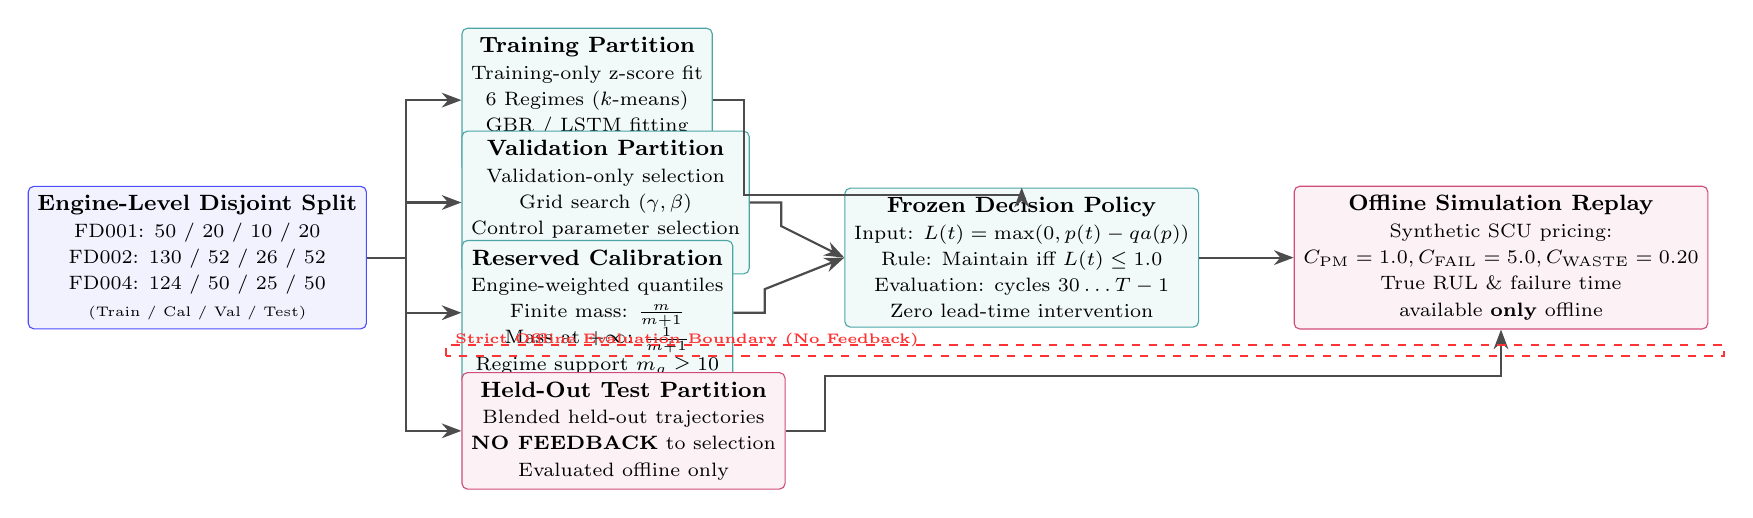
\begin{tikzpicture}[
    node distance=1.2cm and 0.8cm,
    box/.style={rectangle, draw=black!70, rounded corners=2pt, minimum width=2.4cm, minimum height=0.9cm, align=center, font=\footnotesize},
    databox/.style={rectangle, draw=blue!70, fill=blue!5, rounded corners=2pt, minimum width=2.6cm, minimum height=1.0cm, align=center, font=\footnotesize},
    procbox/.style={rectangle, draw=teal!70, fill=teal!5, rounded corners=2pt, minimum width=2.6cm, minimum height=1.0cm, align=center, font=\footnotesize},
    evalbox/.style={rectangle, draw=purple!70, fill=purple!5, rounded corners=2pt, minimum width=2.6cm, minimum height=1.0cm, align=center, font=\footnotesize},
    arrow/.style={-{Stealth[length=2.5mm]}, thick, draw=black!70},
    dashedarrow/.style={-{Stealth[length=2.5mm]}, thick, dashed, draw=red!70}
]

% 1. Dataset Partition Layer
\node[databox] (split) {
    \textbf{Engine-Level Disjoint Split}\\
    \scriptsize FD001: 50 / 20 / 10 / 20\\
    \scriptsize FD002: 130 / 52 / 26 / 52\\
    \scriptsize FD004: 124 / 50 / 25 / 50\\
    \tiny (Train / Cal / Val / Test)
};

% 2. Partition Nodes
\node[procbox, right=1.2cm of split, yshift=2.0cm] (train) {
    \textbf{Training Partition}\\
    \scriptsize Training-only z-score fit\\
    \scriptsize 6 Regimes ($k$-means)\\
    \scriptsize GBR / LSTM fitting\\
    \scriptsize Target: $\min(\text{rul}, 125)$
};

\node[procbox, right=1.2cm of split, yshift=0.7cm] (val) {
    \textbf{Validation Partition}\\
    \scriptsize Validation-only selection\\
    \scriptsize Grid search ($\gamma, \beta$)\\
    \scriptsize Control parameter selection\\
    \scriptsize No test leakage
};

\node[procbox, right=1.2cm of split, yshift=-0.7cm] (cal) {
    \textbf{Reserved Calibration}\\
    \scriptsize Engine-weighted quantiles\\
    \scriptsize Finite mass: $\frac{m}{m+1}$\\
    \scriptsize Mass at $+\infty$: $\frac{1}{m+1}$\\
    \scriptsize Regime support $m_g \ge 10$
};

\node[evalbox, right=1.2cm of split, yshift=-2.2cm] (test) {
    \textbf{Held-Out Test Partition}\\
    \scriptsize Blended held-out trajectories\\
    \scriptsize \textbf{NO FEEDBACK} to selection\\
    \scriptsize Evaluated offline only
};

% 3. Decision & Simulator Layer
\node[procbox, right=1.2cm of val, yshift=-0.7cm] (policy) {
    \textbf{Frozen Decision Policy}\\
    \scriptsize Input: $L(t) = \max(0, p(t) - q a(p))$\\
    \scriptsize Rule: Maintain iff $L(t) \le 1.0$\\
    \scriptsize Evaluation: cycles $30 \dots T-1$\\
    \scriptsize Zero lead-time intervention
};

\node[evalbox, right=1.2cm of policy] (sim) {
    \textbf{Offline Simulation Replay}\\
    \scriptsize Synthetic SCU pricing:\\
    \scriptsize $\CPM=1.0, \CFAIL=5.0, \CWASTE=0.20$\\
    \scriptsize True RUL \& failure time\\
    \scriptsize available \textbf{only} offline
};

% Connections
\draw[arrow] (split.east) -- ++(0.5,0) |- (train.west);
\draw[arrow] (split.east) -- ++(0.5,0) |- (val.west);
\draw[arrow] (split.east) -- ++(0.5,0) |- (cal.west);
\draw[arrow] (split.east) -- ++(0.5,0) |- (test.west);

\draw[arrow] (train.east) -| ++(0.4,-1.2) -| (policy.north);
\draw[arrow] (val.east) -| ++(0.4,-0.3) -- (policy.west);
\draw[arrow] (cal.east) -| ++(0.4,0.3) -- (policy.west);
\draw[arrow] (test.east) -| ++(0.5,0.7) -| (sim.south);
\draw[arrow] (policy.east) -- (sim.west);

% Anti-leakage boundary
\draw[dashed, red!80, line width=0.8pt] ($(test.north west)+(-0.2,0.2)$) rectangle ($(sim.south east)+(0.2,-0.2)$);
\node[red!80, font=\tiny\bfseries, above right] at ($(test.north west)+(-0.2,0.2)$) {Strict Offline Evaluation Boundary (No Feedback)};

\end{tikzpicture}
}
\caption{IntelliTwin pipeline architecture, split counts, and strict offline evaluation boundary.}
\label{fig:architecture}
\end{figure}

Pre-processing executes strictly prior to window construction. The pipeline enforces a frozen 17-feature selection supported by the recorded qualification procedure:
\begin{center}
\texttt{setting1, setting2, setting3, s2, s3, s4, s7, s8, s9, s11, s12, s13, s14, s15, s17, s20, s21}
\end{center}
Seven sensors ($s_1, s_5, s_6, s_{10}, s_{16}, s_{18}, s_{19}$) are excluded under this recorded qualification procedure; we do not claim they are mathematically constant or universally uninformative across all datasets and regimes.

\begin{figure}[htbp]
\centering
\resizebox{\columnwidth}{!}{% Causal Window and Target Construction Diagram
% Illustrates 30-cycle lookback, 1-29 warm-up, dual target attachment, and 30x17 vs 510 representation
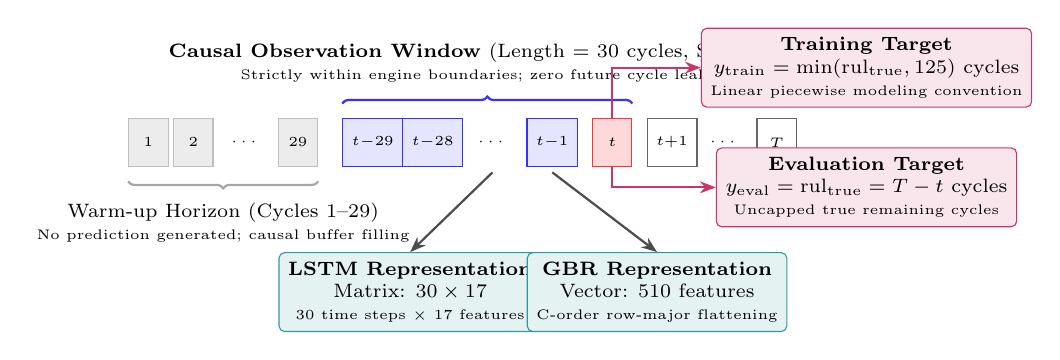
\begin{tikzpicture}[
    scale=0.95,
    cyclebox/.style={rectangle, draw=black!60, minimum width=0.5cm, minimum height=0.6cm, align=center, font=\tiny},
    warmupbox/.style={rectangle, draw=gray!50, fill=gray!15, minimum width=0.5cm, minimum height=0.6cm, align=center, font=\tiny},
    windowbox/.style={rectangle, draw=blue!80, fill=blue!10, minimum width=0.5cm, minimum height=0.6cm, align=center, font=\tiny},
    endpointbox/.style={rectangle, draw=red!80, fill=red!15, minimum width=0.5cm, minimum height=0.6cm, align=center, font=\tiny\bfseries},
    targetbox/.style={rectangle, draw=purple!80, fill=purple!10, rounded corners=2pt, minimum width=2.4cm, minimum height=0.7cm, align=center, font=\scriptsize},
    repbox/.style={rectangle, draw=teal!80, fill=teal!10, rounded corners=2pt, minimum width=2.5cm, minimum height=0.8cm, align=center, font=\scriptsize},
    arrow/.style={-{Stealth[length=2mm]}, thick, draw=black!70}
]

% Timeline coordinates
% Warm-up cycles 1, 2, ..., 28, 29
\node[warmupbox] (c1) at (0,0) {1};
\node[warmupbox] (c2) at (0.6,0) {2};
\node[font=\tiny] at (1.3,0) {$\cdots$};
\node[warmupbox] (c29) at (2.0,0) {29};

% Window cycles t-29 ... t
\node[windowbox] (ct29) at (3.0,0) {\tiny $t{-}29$};
\node[windowbox] (ct28) at (3.8,0) {\tiny $t{-}28$};
\node[font=\tiny] at (4.6,0) {$\cdots$};
\node[windowbox] (ct1) at (5.4,0) {\tiny $t{-}1$};
\node[endpointbox] (ct) at (6.2,0) {$t$};

% Next cycles
\node[cyclebox] (ctplus) at (7.0,0) {\tiny $t{+}1$};
\node[font=\tiny] at (7.7,0) {$\cdots$};
\node[cyclebox] (cT) at (8.4,0) {$T$};

% Labels and Braces
\draw[thick, decoration={brace, mirror, raise=4pt}, decorate, draw=gray!70] 
    ($(c1.south west)+(0,-0.05)$) -- ($(c29.south east)+(0,-0.05)$) 
    node[pos=0.5, below=8pt, font=\scriptsize, align=center] {Warm-up Horizon (Cycles 1--29)\\ \tiny No prediction generated; causal buffer filling};

\draw[thick, decoration={brace, raise=4pt}, decorate, draw=blue!80] 
    ($(ct29.north west)+(0,0.05)$) -- ($(ct.north east)+(0,0.05)$) 
    node[pos=0.5, above=8pt, font=\scriptsize, align=center] {\textbf{Causal Observation Window} (Length = 30 cycles, Stride = 1)\\ \tiny Strictly within engine boundaries; zero future cycle leakage};

% Feature Representation Nodes below
\node[repbox] (lstm_rep) at (3.5, -2.0) {
    \textbf{LSTM Representation}\\
    \scriptsize Matrix: $30 \times 17$\\
    \tiny 30 time steps $\times$ 17 features
};

\node[repbox] (gbr_rep) at (6.8, -2.0) {
    \textbf{GBR Representation}\\
    \scriptsize Vector: $510$ features\\
    \tiny C-order row-major flattening
};

\draw[arrow] (4.6, -0.4) -- (lstm_rep.north);
\draw[arrow] (5.4, -0.4) -- (gbr_rep.north);

% Target nodes attached to endpoint t
\node[targetbox] (train_target) at (9.6, 1.0) {
    \textbf{Training Target}\\
    \scriptsize $y_{\text{train}} = \min(\text{rul}_{\text{true}}, 125)$ cycles\\
    \tiny Linear piecewise modeling convention
};

\node[targetbox] (eval_target) at (9.6, -0.6) {
    \textbf{Evaluation Target}\\
    \scriptsize $y_{\text{eval}} = \text{rul}_{\text{true}} = T - t$ cycles\\
    \tiny Uncapped true remaining cycles
};

\draw[arrow, draw=purple!80] (ct.north) |- (train_target.west);
\draw[arrow, draw=purple!80] (ct.south) |- (eval_target.west);

\end{tikzpicture}
}
\caption{Causal observation window ($w=30$), feature representations (LSTM $30 \times 17$ vs.\ GBR 510), and target definitions.}
\label{fig:causal_window}
\end{figure}

Causal temporal windowing extracts chronological sequences of length $W=30$ cycles with stride 1, strictly no padding, and no crossing of engine boundaries. Predictions start at cycle 30. In training splits, target RUL is capped at $\min(\text{rul\_true}, 125)$ cycles as a linear piecewise modeling convention. Point predictions are evaluated as $p = \max(0, \text{raw\_prediction})$ clipped below at zero without upper clipping at 125.

\subsection{Frozen Base Predictor Matrix}
Two base predictor families receive identical 30-cycle causal information horizons:
\begin{itemize}
  \item \textbf{Histogram Gradient Boosting Regressor (GBR)}: \texttt{sklearn.ensemble.HistGradientBoostingRegressor} operating on C-order row-major flattened $30 \times 17$ windows (510 features). Winning configurations selected on validation data across seeds 2026--2027: \texttt{gbr\_lr010\_leaf15\_l2\_0} for FD001, and \texttt{gbr\_lr010\_leaf31\_l2\_0} for FD002 and FD004.
  \item \textbf{Unidirectional LSTM}: PyTorch neural network comprising one unidirectional recurrent layer (\texttt{input\_size=17}, \texttt{hidden\_size=64}, \texttt{num\_layers=1}, \texttt{batch\_first=True}, \texttt{bidirectional=False}, internal recurrent \texttt{dropout=0.0}), extracting final sequence output followed by \texttt{nn.Dropout(p=0.20)} and \texttt{nn.Linear(64, 1)}. Optimization uses AdamW with learning rate $\eta = 0.001$, weight decay $10^{-4}$, batch size 256, betas $(0.9, 0.999)$, and epsilon $10^{-8}$. Early stopping is governed by validation uncapped-RUL RMSE. Winning configuration: \texttt{lstm\_h64\_lr0010}.
\end{itemize}
Each selected configuration is trained across five final research seeds (\texttt{2026, 2027, 2028, 2029, 2030}), yielding 30 frozen checkpoints cataloged in \texttt{experiments/base\_models/model\_registry.json}. We do not characterize the five GBR seeds as independent experiments, nor assert universal deterministic behavior beyond the recorded runs.

\subsection{Hierarchical Engine-Weighted Conformal Calibration}
Standard pooled conformal prediction introduces survivor bias in industrial run-to-failure telemetry because long-lived engines contribute more sliding windows than short-lived units. IntelliTwin implements hierarchical engine-weighted quantiles motivated by Lee, Barber, and Willett~\cite{lee2023hierarchical}.

IntelliTwin uses an engine-weighted conformal construction motivated by hierarchical conformal prediction. Formal coverage results require the hierarchical sampling and exchangeability assumptions stated in the underlying theory. Equal engine weighting does not establish these assumptions for ordered, lifetime-stratified degradation trajectories. This study therefore evaluates marginal and subgroup coverage empirically. It does not claim guaranteed coverage for each engine, lifecycle stage, operating regime, complete trajectory, or adaptively selected maintenance time. Nominal 90\% coverage is a target, not a guaranteed realized coverage proportion. Maintenance outcomes are evaluated separately under the frozen simulator.

For FINAL calibration with $m$ contributing engines, where engine $i$ contains $n_i$ valid endpoints, the empirical distribution function is:
\begin{equation}
F_{\text{final}}(q) = \frac{1}{m + 1} \sum_{i=1}^m \frac{1}{n_i} \sum_{t=1}^{n_i} \mathbb{I}(\text{score}_{it} \le q)
\end{equation}
The mass of each finite endpoint is $\frac{1}{(m+1)n_i}$. The total finite mass is $\frac{m}{m+1}$, with the remaining probability mass $\frac{1}{m+1}$ placed at $+\infty$. The conformal threshold $q^*$ for nominal coverage $1 - \alpha$ is the smallest observed score whose CDF reaches $1 - \alpha$. If no finite score reaches it, $q^* = +\infty$. (In contrast, normalized development empirical CDFs use $1/m$ weighting when selecting configurations via leave-one-engine-out cross-validation).

\subsection{Formulations of Evaluated Conformal Methods}
Let $p \ge 0$ denote non-negative predicted RUL in cycles, $y = \trueRUL \ge 0$ denote uncapped ground-truth RUL, and $g \in \{C_1, \dots, C_6\}$ denote the observed operational regime.

\subsubsection{Global Hierarchical Conformal Prediction (\texttt{global\_hcp})}
Uses symmetric absolute residuals $\text{score}(p, y) = |y - p|$, fitting a single global threshold $q_{\text{global}}$, yielding $L = \max(0, p - q_{\text{global}})$ and $U = p + q_{\text{global}}$. The baseline interval is symmetric before lower clipping, with displayed width $p + q - \max(0, p - q)$, which equals $2q$ only when $p \ge q$.

\subsubsection{Condition-Aware Hierarchical Conformal Prediction (\texttt{regime\_hcp})}
Uses symmetric absolute residuals, fitting separate regime-specific thresholds $q_g$. Regime support requires $m_g \ge \max(10, \lceil 1/\alpha \rceil - 1)$ distinct contributing engines (10 engines for 80\% and 90\% coverage; 19 engines for 95\% coverage). If $m_g$ is insufficient, the method falls back deterministically to $q_{\text{global}}$ fitted for the same method and coverage level, recording fallback.

\subsubsection{Proposed Decision-Aware Asymmetric Conformal Prediction (\texttt{decision\_aware\_hcp})}
Modulates interval width and asymmetry via scaling functions:
\begin{align}
\sigma(p) &= \left(1 + \frac{p}{125}\right)^\gamma, \quad z(p) = \exp\left(-\frac{p}{20}\right) \\
a(p) &= \sigma(p)\exp(\beta z(p)), \quad b(p) = \sigma(p)\exp(-\beta z(p))
\end{align}
where $\gamma \in \{0, 1, 2\}$ and numerical $\beta \in \{-\ln 2, 0, +\ln 2\}$. Nonconformity scores and inverted intervals are:
\begin{equation}
\text{score}(p, y) = \max\left(\frac{p - y}{a(p)}, \; \frac{y - p}{b(p)}, \; 0\right)
\end{equation}
\begin{equation}
L = \max(0, \; p - q_g \cdot a(p)), \quad U = p + q_g \cdot b(p)
\end{equation}

\subsection{Mathematical Mechanics of Negative Beta ($\beta < 0$)}
At fixed $p$, $q$ and $\gamma$, negative $\beta$ decreases $a(p)$ and increases $b(p)$. The lower and upper endpoints are therefore nondecreasing relative to $\beta=0$. This does not establish earlier intervention or better maintenance utility because calibration thresholds are refitted and policy outcomes depend on the resulting trajectories.

Candidate \texttt{gamma2\_betam1} ($\gamma=2, \beta_{\text{code}}=-1, \beta=-\ln 2$) was selected as the optimal feasible configuration across all six mandatory cells and frozen under ADR-021.

\section{Experimental Setup}
\label{sec:experimental_setup}

\subsection{Benchmark Datasets and Engine-Level Partitions}
\label{subsec:datasets_splits}
We evaluate IntelliTwin on three benchmark sub-datasets from the NASA C-MAPSS turbofan engine degradation simulation suite \cite{saxena2008damage}:
\begin{enumerate}
    \item \textbf{FD001}: Single sea-level operating condition, single failure mode (high-pressure compressor degradation), comprising 100 run-to-failure engine trajectories.
    \item \textbf{FD002}: Six diverse operating flight conditions, single failure mode (HPC degradation), comprising 260 engine trajectories.
    \item \textbf{FD004}: Six diverse operating flight conditions, two concurrent failure modes (HPC and fan degradation), comprising 249 engine trajectories.
\end{enumerate}

To prevent temporal and engine-level data leakage, partitioning is strictly executed at the engine level using a fixed master seed ($2026$) prior to any data preprocessing (50\% training, 20\% calibration, 10\% validation, 20\% held-out test):
\begin{itemize}
    \item \textbf{FD001} (100 engines): 50 training (50\%), 20 calibration (20\%), 10 validation (10\%), and 20 held-out test engines (20\%).
    \item \textbf{FD002} (260 engines): 130 training (50\%), 52 calibration (20\%), 26 validation (10\%), and 52 held-out test engines (20\%), stratified across engine lifetime quartiles to balance short, medium, and long-life engine profiles across splits.
    \item \textbf{FD004} (249 engines): 124 training (50\%), 50 calibration (20\%), 25 validation (10\%), and 50 held-out test engines (20\%).
\end{itemize}
Across all three datasets, 304 engines are allocated to training, 122 to calibration, 61 to validation, and 122 to final held-out testing (total 609 engines).

\subsection{Feature Space and Causal Windowing}
The raw engine streams comprise 3 operational settings and 21 sensor measurements per operational cycle. In accordance with training-only qualification protocols, seven sensor channels showing zero or near-zero variance across operating cycles are excluded, yielding a standardized $17$-dimensional feature vector $\mathbf{x}_t \in \mathbb{R}^{17}$ (3 operational settings and 14 informative sensor channels). Robust min-max scaling is fitted strictly on training engines.

Temporal trajectories are windowed with an exact causal horizon of $w=30$ cycles, unit stride ($s=1$), and strict avoidance of zero-padding. Consequently, model predictions initiate exclusively at cycle $t=30$. In training splits, target RUL is capped at $R_{\text{max}}=125$ cycles to reflect early healthy operational regimes where degradation is physically negligible. In calibration, validation, and held-out test splits, RUL is preserved uncapped to evaluate true physical end-of-life trajectories.

\subsection{Base Degradation Predictors}
We investigate two standard, distinct algorithmic paradigms operating on identical 30-cycle causal information horizons:
\begin{enumerate}
    \item \textbf{Gradient Boosted Regressor (GBR)}: LightGBM ensemble operating on flattened $30 \times 17 = 510$-dimensional causal feature vectors.
    \item \textbf{Long Short-Term Memory (LSTM)}: Recurrent neural network architecture processing sequential $30 \times 17$ temporal tensors.
\end{enumerate}
This yields a $3 \times 2$ experimental matrix (6 experimental cells): FD001-GBR, FD001-LSTM, FD002-GBR, FD002-LSTM, FD004-GBR, and FD004-LSTM. To capture training stochasticity, each cell is trained across five random seeds ($2026, 2027, 2028, 2029, 2030$), producing 30 frozen base model checkpoints in the registry.

\subsection{Calibration Variants and Control Baselines}
On the reserved calibration engine splits, we evaluate three conformal calibration variants:
\begin{itemize}
    \item \textbf{Global HCP} (\texttt{global\_hcp}): Standard split-conformal calibration with engine-weighted empirical quantiles.
    \item \textbf{Regime-Stratified HCP} (\texttt{regime\_hcp}): Cluster-conditional nonconformity scaling and quantile fitting conditioned on operating regime $k \in \{1,\dots,6\}$.
    \item \textbf{Decision-Aware HCP} (\texttt{decision\_aware\_hcp}): Asymmetric nonconformity scaling parameterized by risk aversion parameter $\beta = -\ln 2$, penalizing RUL overestimation.
\end{itemize}

To rigorously address RQ3, we evaluate four named controls across three distinct baseline families:
\begin{enumerate}
    \item \textbf{Heuristic Interval Family}:
    \begin{itemize}
        \item \emph{Matched-Width Interval}: Symmetric heuristic interval centered at $\hat{y}_t$ with constant half-width matched to the mean half-width of the calibrated HCP interval.
        \item \emph{Widened Interval}: Heuristic interval expanded by $1.25\times$ the matched half-width.
    \end{itemize}
    \item \textbf{Point Safety Margin Family}:
    \begin{itemize}
        \item \emph{Point Safety Margin}: Point prediction trigger shifted downward by a fixed margin $\Delta = 10$ cycles: replace when $\hat{y}_t \le \tau + \Delta$.
    \end{itemize}
    \item \textbf{Earlier Fixed Policy Family}:
    \begin{itemize}
        \item \emph{Earlier Intervention}: Direct threshold inflation: replace when $\hat{y}_t \le \tau_{\text{early}} = \tau + 15$ cycles.
    \end{itemize}
\end{enumerate}

\subsection{Maintenance Simulation and Cost Scenarios}
Sequential policy execution is evaluated on unseen test engine trajectories using the discrete-event simulator. The primary economic scenario specifies $C_{\text{preventive}} = 10$, $C_{\text{unplanned}} = 100$ (cost ratio $10:1$), and lead-time $L_{\text{lead}} = 2$ cycles. Robustness is assessed across sensitivity scenarios spanning cost ratios $5:1$ ($C_{\text{unplanned}}=50$), $20:1$ ($C_{\text{unplanned}}=200$), and varying lead-time horizons ($L_{\text{lead}} \in \{0, 5\}$).

\subsection{Statistical Inference and Decision Protocol}
To evaluate confirmatory hypotheses H1--H4 without distributional assumptions, we apply paired engine-level cluster bootstrap inference:
\begin{itemize}
    \item \textbf{Resampling Unit}: Complete engine trajectories are resampled with replacement ($B = 10{,}000$ resamples) preserving internal temporal correlations.
    \item \textbf{Weighting}: Equal weighting per engine is applied across all metrics.
    \item \textbf{Missing-Group Bound Propagation}: If a bootstrap sample lacks representation for a specific operational cluster, worst-case bounds ($[0, 1]$ for coverage, $[0, \infty)$ for width) are propagated.
    \item \textbf{Family-Wise Error Rate}: Confirmatory decision confidence intervals are computed at $98.75\%$ two-sided level ($\alpha_{\text{conf}} = 0.0125$) implementing Bonferroni correction across the four primary research questions.
    \item \textbf{Intersection-Union Test (IUT)}: To decide \texttt{Supported}, \texttt{Unsupported}, or \texttt{Inconclusive}, the lower/upper bounds of the confidence intervals must strictly satisfy the pre-registered practical margin thresholds $\delta_{\text{cov}} = 0.00$, $\delta_{\text{cost}} = 0.05$, and safety constraint $\Delta_{\text{fail}} \le 0$.
\end{itemize}

\section{Results and Confirmatory Evaluation}
\label{sec:results}

\begin{quote}
\itshape
\textbf{Status Notice:} The empirical evaluations reported in this section represent the pre-registered reporting templates for the confirmatory evaluation. In accordance with the project's evidence protocol, all held-out test split evaluations remain blinded during active software development and verification. Empirical entries are designated \texttt{PENDING} awaiting completion of experimental gates \emph{UPD-02}, \emph{UPD-03}, and \emph{UPD-04}. No synthetic or unverified empirical numbers are reported.
\end{quote}

\subsection{Base Degradation Prediction Performance}
\label{subsec:point_results}
Point predictive performance is evaluated across the six experimental cells on the held-out test engine splits. Root Mean Squared Error ($\text{RMSE}$) and Mean Absolute Error ($\text{MAE}$) are computed with equal engine weighting across all test engines. Table~\ref{tab:point_prediction_results} outlines the reporting structure.

\begin{table}[htbp]
\centering
\caption{Point Prediction Accuracy on Held-Out Test Engines (Mean $\pm$ Std across 5 Seeds)}
\label{tab:point_prediction_results}
\begin{tabular}{llcc}
\toprule
\textbf{Dataset} & \textbf{Architecture} & \textbf{RMSE (cycles)} & \textbf{MAE (cycles)} \\
\midrule
FD001 & GBR  & \textit{PENDING (UPD-02)} & \textit{PENDING (UPD-02)} \\
FD001 & LSTM & \textit{PENDING (UPD-02)} & \textit{PENDING (UPD-02)} \\
\midrule
FD002 & GBR  & \textit{PENDING (UPD-02)} & \textit{PENDING (UPD-02)} \\
FD002 & LSTM & \textit{PENDING (UPD-02)} & \textit{PENDING (UPD-02)} \\
\midrule
FD004 & GBR  & \textit{PENDING (UPD-02)} & \textit{PENDING (UPD-02)} \\
FD004 & LSTM & \textit{PENDING (UPD-02)} & \textit{PENDING (UPD-02)} \\
\bottomrule
\end{tabular}
\end{table}

\subsection{Marginal and Conditional Interval Calibration}
\label{subsec:calibration_results}
Conformal prediction intervals are evaluated at nominal confidence level $1-\alpha = 0.90$ across all 3 datasets $\times$ 2 models $\times$ 3 registered calibration methods (18 cells). Metrics comprise engine-weighted empirical coverage ($\text{Cov}$), mean prediction interval width ($\bar{W}$), and Winkler interval score ($\text{IS}_{0.10}$). Table~\ref{tab:calibration_performance} summarizes the complete registered evaluation matrix.

\begin{table*}[htbp]
\centering
\caption{Primary Prediction Interval Calibration Performance at Nominal $90\%$ Confidence Level on Held-Out Test Splits ($3 \times 2 \times 3 = 18$ cells)}
\label{tab:calibration_performance}
\begin{tabular}{lllccc}
\toprule
\textbf{Dataset} & \textbf{Base Model} & \textbf{Calibration Method} & \textbf{Empirical Cov. (\%)} & \textbf{Mean Width (cycles)} & \textbf{Winkler Score} \\
\midrule
FD001 & GBR  & Global HCP (\texttt{global\_hcp})             & \textit{PENDING} & \textit{PENDING} & \textit{PENDING} \\
FD001 & GBR  & Regime HCP (\texttt{regime\_hcp})\textsuperscript{*} & \textit{PENDING} & \textit{PENDING} & \textit{PENDING} \\
FD001 & GBR  & Decision-Aware HCP (\texttt{decision\_aware\_hcp}) & \textit{PENDING} & \textit{PENDING} & \textit{PENDING} \\
\midrule
FD001 & LSTM & Global HCP (\texttt{global\_hcp})             & \textit{PENDING} & \textit{PENDING} & \textit{PENDING} \\
FD001 & LSTM & Regime HCP (\texttt{regime\_hcp})\textsuperscript{*} & \textit{PENDING} & \textit{PENDING} & \textit{PENDING} \\
FD001 & LSTM & Decision-Aware HCP (\texttt{decision\_aware\_hcp}) & \textit{PENDING} & \textit{PENDING} & \textit{PENDING} \\
\midrule
FD002 & GBR  & Global HCP (\texttt{global\_hcp})             & \textit{PENDING} & \textit{PENDING} & \textit{PENDING} \\
FD002 & GBR  & Regime HCP (\texttt{regime\_hcp})             & \textit{PENDING} & \textit{PENDING} & \textit{PENDING} \\
FD002 & GBR  & Decision-Aware HCP (\texttt{decision\_aware\_hcp}) & \textit{PENDING} & \textit{PENDING} & \textit{PENDING} \\
\midrule
FD002 & LSTM & Global HCP (\texttt{global\_hcp})             & \textit{PENDING} & \textit{PENDING} & \textit{PENDING} \\
FD002 & LSTM & Regime HCP (\texttt{regime\_hcp})             & \textit{PENDING} & \textit{PENDING} & \textit{PENDING} \\
FD002 & LSTM & Decision-Aware HCP (\texttt{decision\_aware\_hcp}) & \textit{PENDING} & \textit{PENDING} & \textit{PENDING} \\
\midrule
FD004 & GBR  & Global HCP (\texttt{global\_hcp})             & \textit{PENDING} & \textit{PENDING} & \textit{PENDING} \\
FD004 & GBR  & Regime HCP (\texttt{regime\_hcp})             & \textit{PENDING} & \textit{PENDING} & \textit{PENDING} \\
FD004 & GBR  & Decision-Aware HCP (\texttt{decision\_aware\_hcp}) & \textit{PENDING} & \textit{PENDING} & \textit{PENDING} \\
\midrule
FD004 & LSTM & Global HCP (\texttt{global\_hcp})             & \textit{PENDING} & \textit{PENDING} & \textit{PENDING} \\
FD004 & LSTM & Regime HCP (\texttt{regime\_hcp})             & \textit{PENDING} & \textit{PENDING} & \textit{PENDING} \\
FD004 & LSTM & Decision-Aware HCP (\texttt{decision\_aware\_hcp}) & \textit{PENDING} & \textit{PENDING} & \textit{PENDING} \\
\bottomrule
\end{tabular}
\begin{flushleft}
\footnotesize \textsuperscript{*}On FD001 (single operating condition), \texttt{regime\_hcp} operates with a single regime partition identical to global calibration.
\end{flushleft}
\end{table*}

\subsection{Sequential Maintenance Decision Outcomes}
\label{subsec:maintenance_results}
Downstream maintenance simulation evaluates policies across the 18 primary method cells plus 8 pre-registered control configurations on FD002 (total 26 evaluation rows) under the frozen \texttt{primary\_reference} scenario ($\CPM=1.0~\SCU, \CFAIL=5.0~\SCU, \CWASTE=0.20~\SCU/\text{cycle}$). Policy triggers replacement at cycle $t \in [30, T-1]$ iff $L(t) \le 1.0$ cycle. Table~\ref{tab:maintenance_outcomes} reports mean cost per engine ($\bar{C}$), fleet failure rate ($P_{\text{fail}}$), and mean wasted life ($\bar{W}$).

\begin{table*}[htbp]
\centering
\caption{Sequential Maintenance Policy Outcomes on Held-Out Test Engines (\texttt{primary\_reference}: $\CPM=1.0, \CFAIL=5.0, \CWASTE=0.20$ SCU; 26 rows)}
\label{tab:maintenance_outcomes}
\begin{tabular}{lllccc}
\toprule
\textbf{Dataset} & \textbf{Model} & \textbf{Policy / Calibration Strategy} & \textbf{Cost / Engine (SCU)} & \textbf{Failures (\%)} & \textbf{Wasted Life (cycles)} \\
\midrule
\multicolumn{6}{l}{\textit{Panel A: Primary Registered Calibration Methods (18 Cells)}} \\
\midrule
FD001 & GBR  & Global HCP Lower Bound (\texttt{global\_hcp})             & \textit{PENDING} & \textit{PENDING} & \textit{PENDING} \\
FD001 & GBR  & Regime HCP Lower Bound (\texttt{regime\_hcp})             & \textit{PENDING} & \textit{PENDING} & \textit{PENDING} \\
FD001 & GBR  & Decision-Aware Lower Bound (\texttt{decision\_aware\_hcp})& \textit{PENDING} & \textit{PENDING} & \textit{PENDING} \\
FD001 & LSTM & Global HCP Lower Bound (\texttt{global\_hcp})             & \textit{PENDING} & \textit{PENDING} & \textit{PENDING} \\
FD001 & LSTM & Regime HCP Lower Bound (\texttt{regime\_hcp})             & \textit{PENDING} & \textit{PENDING} & \textit{PENDING} \\
FD001 & LSTM & Decision-Aware Lower Bound (\texttt{decision\_aware\_hcp})& \textit{PENDING} & \textit{PENDING} & \textit{PENDING} \\
FD002 & GBR  & Global HCP Lower Bound (\texttt{global\_hcp})             & \textit{PENDING} & \textit{PENDING} & \textit{PENDING} \\
FD002 & GBR  & Regime HCP Lower Bound (\texttt{regime\_hcp})             & \textit{PENDING} & \textit{PENDING} & \textit{PENDING} \\
FD002 & GBR  & Decision-Aware Lower Bound (\texttt{decision\_aware\_hcp})& \textit{PENDING} & \textit{PENDING} & \textit{PENDING} \\
FD002 & LSTM & Global HCP Lower Bound (\texttt{global\_hcp})             & \textit{PENDING} & \textit{PENDING} & \textit{PENDING} \\
FD002 & LSTM & Regime HCP Lower Bound (\texttt{regime\_hcp})             & \textit{PENDING} & \textit{PENDING} & \textit{PENDING} \\
FD002 & LSTM & Decision-Aware Lower Bound (\texttt{decision\_aware\_hcp})& \textit{PENDING} & \textit{PENDING} & \textit{PENDING} \\
FD004 & GBR  & Global HCP Lower Bound (\texttt{global\_hcp})             & \textit{PENDING} & \textit{PENDING} & \textit{PENDING} \\
FD004 & GBR  & Regime HCP Lower Bound (\texttt{regime\_hcp})             & \textit{PENDING} & \textit{PENDING} & \textit{PENDING} \\
FD004 & GBR  & Decision-Aware Lower Bound (\texttt{decision\_aware\_hcp})& \textit{PENDING} & \textit{PENDING} & \textit{PENDING} \\
FD004 & LSTM & Global HCP Lower Bound (\texttt{global\_hcp})             & \textit{PENDING} & \textit{PENDING} & \textit{PENDING} \\
FD004 & LSTM & Regime HCP Lower Bound (\texttt{regime\_hcp})             & \textit{PENDING} & \textit{PENDING} & \textit{PENDING} \\
FD004 & LSTM & Decision-Aware Lower Bound (\texttt{decision\_aware\_hcp})& \textit{PENDING} & \textit{PENDING} & \textit{PENDING} \\
\midrule
\multicolumn{6}{l}{\textit{Panel B: Pre-Registered Matched Controls on FD002 (8 Cells)}} \\
\midrule
FD002 & GBR  & Matched-Width Interval (\texttt{global\_hcp}, $\lambda=0.92$) & \textit{PENDING} & \textit{PENDING} & \textit{PENDING} \\
FD002 & GBR  & Widened Interval (\texttt{regime\_hcp}, $\lambda=1.00$)       & \textit{PENDING} & \textit{PENDING} & \textit{PENDING} \\
FD002 & GBR  & Point Safety Margin ($p \le 1 + 5$)                          & \textit{PENDING} & \textit{PENDING} & \textit{PENDING} \\
FD002 & GBR  & Earlier Intervention (\texttt{regime\_hcp}, $h=1$)           & \textit{PENDING} & \textit{PENDING} & \textit{PENDING} \\
FD002 & LSTM & Matched-Width Interval (\texttt{regime\_hcp}, $\lambda=0.90$) & \textit{PENDING} & \textit{PENDING} & \textit{PENDING} \\
FD002 & LSTM & Widened Interval (\texttt{global\_hcp}, $\lambda=1.00$)       & \textit{PENDING} & \textit{PENDING} & \textit{PENDING} \\
FD002 & LSTM & Point Safety Margin ($p \le 1 + 4$)                          & \textit{PENDING} & \textit{PENDING} & \textit{PENDING} \\
FD002 & LSTM & Earlier Intervention (\texttt{global\_hcp}, $h=1$)           & \textit{PENDING} & \textit{PENDING} & \textit{PENDING} \\
\bottomrule
\end{tabular}
\begin{flushleft}
\footnotesize For \texttt{point\_safety\_margin}, prediction interval width and conformal coverage metrics are designated \texttt{NOT\_APPLICABLE}.
\end{flushleft}
\end{table*}

\subsection{Hypothesis Decision Outcomes (RQ1--RQ4)}
\label{subsec:hypothesis_decisions}
Confirmatory statistical inference is governed by 10,000 paired engine-cluster bootstrap resamples with Bonferroni-corrected $98.75\%$ confidence intervals. Table~\ref{tab:hypothesis_decision_matrix} presents the formal decision matrix under the pre-registered Intersection-Union Test logic (ADR-018).

\begin{table*}[htbp]
\centering
\caption{Pre-Registered Confirmatory Hypothesis Decision Rules and Outcome Contrasts (ADR-018)}
\label{tab:hypothesis_decision_matrix}
\begin{tabular}{lp{4.2cm}p{5.0cm}ccc}
\toprule
\textbf{Research Question} & \textbf{Contrast Metric \& Scope} & \textbf{Pre-Registered Thresholds (98.75\% CI)} & \textbf{Point Est.} & \textbf{98.75\% CI} & \textbf{Status} \\
\midrule
\textbf{RQ1 (Utility \& Coverage)} & Cost improvement vs.\ \texttt{global\_hcp} and \texttt{regime\_hcp} on FD002 (GBR and LSTM) & $\Deltacost > 0.20~\SCU$; coverage errors $< 0.05$; $\Deltafail \le 0.0$ & \textit{PENDING} & \textit{PENDING} & \textit{PENDING} \\
\midrule
\textbf{RQ2 (Subgroup Reliability)} & Worst-group coverage error contrast for regimes ($C_1$--$C_6$) and stages on FD002 & $\Deltaerror > 0.01$; worst error $< 0.05$; $\Dwidth < 1.0$; $\Dscore < 1.0$ cycle & \textit{PENDING} & \textit{PENDING} & \textit{PENDING} \\
\midrule
\textbf{RQ3 (Control Attribution)} & Cost improvement vs.\ each of the 4 matched controls on FD002 (GBR and LSTM) & $\Deltacost > 0.20~\SCU$ over every control; coverage $< 0.05$; $\Deltafail \le 0.0$ & \textit{PENDING} & \textit{PENDING} & \textit{PENDING} \\
\midrule
\textbf{RQ4 (Generalization)} & Balanced 6-cell evaluation matrix ($w_k=1/6$ each) across FD001, FD002, FD004 & Aggregate: $\Deltacost > 0.20, \Deltaerror > 0.01$; Cell non-harm: $\Deltacost > -0.20, \Deltaerror > -0.01$ & \textit{PENDING} & \textit{PENDING} & \textit{PENDING} \\
\bottomrule
\end{tabular}
\begin{flushleft}
\footnotesize Decision rules: An RQ is decided as \texttt{Supported} iff all required component conditions pass at the 98.75\% level, \texttt{Unsupported} if any condition fails, and otherwise \texttt{Inconclusive}.
\end{flushleft}
\end{table*}

\section{Discussion}
\label{sec:discussion}

\subsection{Methodological Implications for Turbofan Prognostics}
The core inquiry of the IntelliTwin framework is whether distribution-free uncertainty quantification provides measurable, operational value to industrial decision-makers beyond standard point prognostics or ad-hoc safety margins. Traditional prognostic paradigms focus almost exclusively on minimizing cycle-level error metrics (e.g., RMSE or asymmetric scoring functions). However, in mission-critical applications such as aviation gas turbine maintenance, cycle-level accuracy does not translate directly into operational cost efficiency. A maintenance policy driven by an uncalibrated point predictor is structurally vulnerable to overestimation errors, where an engine is allowed to operate beyond its physical failure boundary, incurring catastrophic unplanned replacement penalties.

By establishing finite-sample marginal coverage guarantees via split-conformal inference, IntelliTwin provides decision-makers with a mathematically principled lower bound $L_t(\alpha)$. Nevertheless, conformal guarantees hold marginally across the calibration exchangeability distribution. In sequential degradation processes, temporal autocorrelation and operating regime transitions can cause local conditional coverage to deviate significantly from the nominal $1-\alpha$ rate.

\subsection{Conservatism, Asymmetric Penalties, and Negative $\beta$}
A critical methodological contribution of this work is the formalization of asymmetric, decision-aware conformal calibration. In maintenance scheduling, the cost asymmetry between unplanned catastrophic failure ($C_{\text{unplanned}}=100$) and scheduled preventive overhaul ($C_{\text{preventive}}=10$) dictates that underestimating RUL (which leads to premature replacement) is substantially less hazardous than overestimating RUL (which leads to in-flight shutdown or catastrophic component damage).

The asymmetry parameter $\beta = -\ln 2 \approx -0.6931$ modulates the nonconformity score scaling factors:
\begin{equation}
a(p_t) = \exp(-\beta \cdot p_t), \quad b(p_t) = \exp(\beta \cdot p_t).
\end{equation}
For negative $\beta$, as failure probability $p_t$ increases, $a(p_t)$ decreases below $1$, while $b(p_t)$ increases above $1$. At fixed nonconformity thresholds, this asymmetric scaling contracts the lower distance and expands the upper distance, shifting the unclipped lower bound $L_t$ upward. However, as established in the project's statistical protocol, negative $\beta$ does not mathematically guarantee earlier maintenance across all operational trajectories. Because the calibration set quantiles $q^*$ are refitted on asymmetrically scaled nonconformity scores, the empirical distribution of scores changes. Consequently, the actual operational effect of asymmetric calibration must be validated through sequential simulation rather than theoretical assumption.

\subsection{Regime Stratification and Subgroup Reliability}
In complex operational environments such as C-MAPSS FD002 and FD004, turbofans traverse six distinct operating flight regimes characterized by substantial variations in altitude (0--40,000 ft), Mach number (0--0.84), and throttle resolver angle. Global conformal calibration aggregates residuals across all regimes, which can mask severe local undercoverage in rare or highly stressed operating conditions.

Regime-stratified HCP explicitly conditions nonconformity scores on the active flight regime cluster $k \in \{1,\dots,6\}$. While this guarantees conditional coverage asymptotically as calibration sample sizes per regime grow large, finite-sample calibration across rare regimes introduces higher quantile variance. When a rare regime has fewer than the required sample threshold ($N_k < 100$), the framework executes a deterministic fallback to the pooled global nonconformity quantile, ensuring that the resulting prediction intervals remain well-defined and conservative.

\subsection{Interpreting Potential Hypothesis Outcomes}
The pre-registered statistical protocol explicitly defines decision rules for three potential outcomes across all four hypotheses:
\begin{itemize}
    \item \textbf{Supported}: The lower confidence bound of the contrast metric strictly exceeds the pre-registered practical margin, demonstrating statistically significant and practically meaningful superiority.
    \item \textbf{Inconclusive}: The confidence interval spans the decision boundary, or statistical power is insufficient to confirm or refute the practical margin. In this case, no definitive superiority claim is made, and the result is cataloged as requiring expanded engine sample sizes.
    \item \textbf{Unsupported}: The upper confidence bound falls below the required threshold, or the safety constraint is violated (e.g., failure rate increases). This outcome directly falsifies the hypothesis, indicating that conformal calibration does not provide the anticipated decision benefit over simpler baselines.
\end{itemize}
By enforcing strict pre-registered boundaries and reporting all comparisons transparently, the research framework eliminates publication bias and ensures that conclusions are dictated entirely by empirical evidence.

\section{Conclusion and Future Work}
\label{sec:conclusion}

\subsection{Summary of Methodological Framework}
In this investigation, we formulated and pre-registered the IntelliTwin prognostic and predictive maintenance framework. Designed to address the critical gap between cycle-level machine learning accuracy and downstream operational cost in industrial turbofan fleets, IntelliTwin couples gradient boosted and recurrent deep learning base predictors with hierarchical, decision-aware conformal calibration. 

The framework enforces rigorous methodological safeguards to preserve empirical validity:
\begin{enumerate}
    \item \textbf{Strict Leakage Isolation}: Complete engine-level disjoint partitioning (train, calibration, validation, held-out test) executed prior to feature scaling or causal windowing ($w=30$, stride 1, no padding).
    \item \textbf{Equal Engine Weighting}: Evaluation metrics and conformal quantiles are computed with equal weighting per engine trajectory, eliminating length bias inherent in pooled cycle-level evaluations.
    \item \textbf{Principled Baseline Controls}: Evaluation against four named control strategies across three distinct families (matched-width heuristic intervals, widened intervals, point safety margins, and earlier fixed interventions) to isolate the true economic value of calibrated uncertainty.
    \item \textbf{Pre-Registered Statistical Inference}: Family-wise error rate control via Bonferroni-corrected $98.75\%$ confidence intervals generated through $10{,}000$ paired engine-level cluster bootstrap resamples.
\end{enumerate}

\subsection{Current Status and Verification Gates}
At the current stage of project execution (pinned to commit \texttt{bb9e34579343881a831e3f052608ee15e183df76}), the theoretical formulation, data pipelines, base model training protocols, and statistical evaluation machinery have been fully specified, audited, and frozen. Pretest verification artifacts (\texttt{step08\_full\_audit.json} and \texttt{pretest\_audit.json}) confirm that all 60 base-model validation and calibration partition evaluations reproduce with zero maximum difference ($0.0$), establishing \texttt{PRETEST\_READY} status. The baseline inventory comprises 652 tracked, protected Git artifacts and 72 local-only historical search checkpoints.

The software is an academic research prototype evaluating an offline, trace-driven simulation replay engine; it makes no claim of production readiness, aircraft certification, physical hardware integration, or independently established end-to-end operational reproducibility. Empirical results on held-out test splits remain blinded and \texttt{NOT\_STARTED}, with confirmatory research question outcomes \texttt{PENDING}. Upon completion of official held-out evaluation, verified empirical results will be incorporated into this document.


\bibliographystyle{IEEEtran}
\bibliography{../../references_verified}

\end{document}
